\section{Travessias em árvores}

\begin{frame}[fragile]{DFS em árvores}

    \begin{itemize}
        \item Embora a DFS e a BFS possa ser utilizadas em árvores sem nenhuma alteração,
            a estrutura simplificada da árvore permite implementações mais simples e com
            menor complexidade de memória
            
        \item Por conta da ausência de ciclos, a implementação da DFS em árvores dispensa o
            vetor que mantém o registro dos vértices já visitados

        \item Ele pode ser substituído por um parâmetro extra, que mantém o registro do nó $p$ que
            antecede $u$ na travessia

        \item Assim, a complexidade de memória reduz de $O(V)$ para $O(1)$

        \item Na primeira chamada da DFS, o parâmetro $p$ deve ser igual a zero (ou qualquer
            valor sentinela que não seja um rótulo de um dos vértices do grafo)
    \end{itemize}

\end{frame}

\begin{frame}[fragile]{Implementação da DFS em árvores}
    \inputsnippet{c++}{1}{17}{tree_dfs.cpp}
\end{frame}

\begin{frame}[fragile]{Implementação da DFS em árvores}
    \inputsnippet{c++}{18}{38}{tree_dfs.cpp}
\end{frame}

\begin{frame}[fragile]{Números de nós na subárvore}

    \begin{itemize}
        \item A DFS, em conjunto com técnicas de programação dinâmica, permite computar em
            $O(N)$ algumas características da árvore

        \item Um primeiro exemplo seria o número de nós  \code{c}{nodes[u]} da subárvore cuja raiz 
        é o nó $u$

        \item Se $u$ é uma folha, então \code{c}{nodes[u]} = 1 (apenas $u$ faz parte da subárvore)

        \item Caso contrário, \code{c}{nodes[u]} = 1 + $\sum_v$\code{c}{nodes[v]}, onde 
        $v$ é um filho de $u$

    \end{itemize}

\end{frame}

\begin{frame}[fragile]{Visualização do algoritmo que computa o número de nós}

    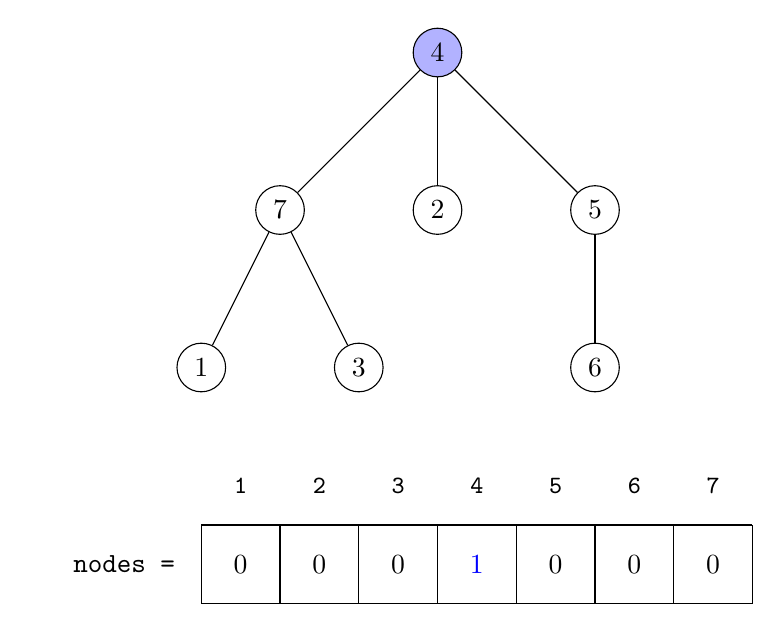
\begin{tikzpicture}

        \begin{scope}{shift={(3,0)}}
            \node[opacity=0] (X) at (-1, 0) { $1$ };

            \node[fill=blue!30,circle,draw] (D) at (4, 5) { $4$ };
            \node[circle,draw] (C) at (2, 3) { $7$ };
            \node[circle,draw,fill=white!30] (E) at (4, 3) { $2$ };
            \node[circle,draw] (F) at (6, 3) { $5$ };
            \node[circle,draw,fill=white!30] (A) at (1, 1) { $1$ };
            \node[circle,draw,fill=white!30] (B) at (3, 1) { $3$ };
            \node[circle,draw,fill=white!30] (G) at (6, 1) { $6$ };

            \draw (A) -- (C);
            \draw (B) -- (C);
            \draw (C) -- (D);
            \draw (D) -- (E);
            \draw (D) -- (F);
            \draw (F) -- (G);

            \node[anchor=west] at (-0.75, -1.5) { \texttt{nodes = } };
            \draw (1, -2) grid (8, -1);

            \node at (1.5, -0.5) { \small \texttt{1} };
            \node at (2.5, -0.5) { \small \texttt{2} };
            \node at (3.5, -0.5) { \small \texttt{3} };
            \node at (4.5, -0.5) { \small \texttt{4} };
            \node at (5.5, -0.5) { \small \texttt{5} };
            \node at (6.5, -0.5) { \small \texttt{6} };
            \node at (7.5, -0.5) { \small \texttt{7} };

            \node at (1.5, -1.5) { $0$ };
            \node at (2.5, -1.5) { $0$ };
            \node at (3.5, -1.5) { $0$ };
            \node at (4.5, -1.5) { \textcolor{blue}{$1$} };
            \node at (5.5, -1.5) { $0$ };
            \node at (6.5, -1.5) { $0$ };
            \node at (7.5, -1.5) { $0$ };

        \end{scope}
    \end{tikzpicture}

\end{frame}

\begin{frame}[fragile]{Visualização do algoritmo que computa o número de nós}

    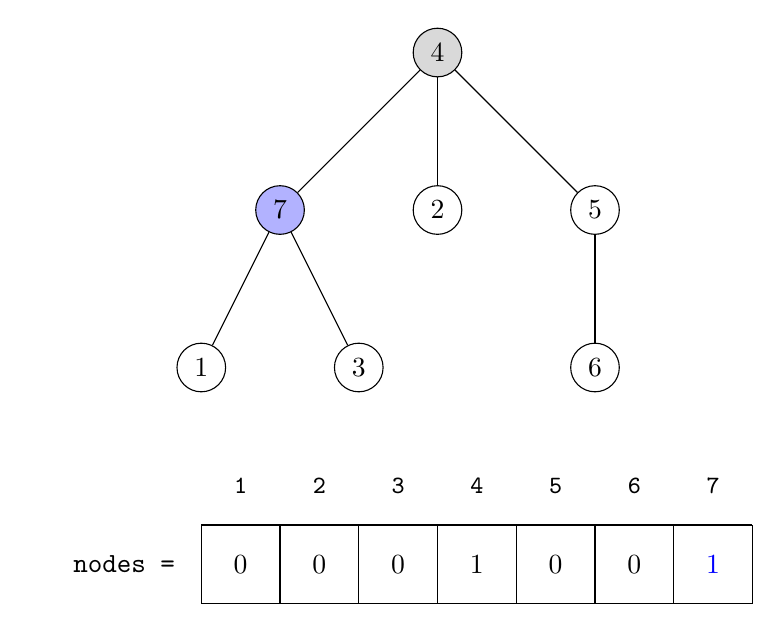
\begin{tikzpicture}

        \begin{scope}{shift={(3,0)}}
            \node[opacity=0] (X) at (-1, 0) { $1$ };

            \node[fill=gray!30,circle,draw] (D) at (4, 5) { $4$ };
            \node[circle,draw,fill=blue!30] (C) at (2, 3) { $7$ };
            \node[circle,draw,fill=white!30] (E) at (4, 3) { $2$ };
            \node[circle,draw] (F) at (6, 3) { $5$ };
            \node[circle,draw,fill=white!30] (A) at (1, 1) { $1$ };
            \node[circle,draw,fill=white!30] (B) at (3, 1) { $3$ };
            \node[circle,draw,fill=white!30] (G) at (6, 1) { $6$ };

            \draw (A) -- (C);
            \draw (B) -- (C);
            \draw (C) -- (D);
            \draw (D) -- (E);
            \draw (D) -- (F);
            \draw (F) -- (G);

            \node[anchor=west] at (-0.75, -1.5) { \texttt{nodes = } };
            \draw (1, -2) grid (8, -1);

            \node at (1.5, -0.5) { \small \texttt{1} };
            \node at (2.5, -0.5) { \small \texttt{2} };
            \node at (3.5, -0.5) { \small \texttt{3} };
            \node at (4.5, -0.5) { \small \texttt{4} };
            \node at (5.5, -0.5) { \small \texttt{5} };
            \node at (6.5, -0.5) { \small \texttt{6} };
            \node at (7.5, -0.5) { \small \texttt{7} };

            \node at (1.5, -1.5) { $0$ };
            \node at (2.5, -1.5) { $0$ };
            \node at (3.5, -1.5) { $0$ };
            \node at (4.5, -1.5) { $1$ };
            \node at (5.5, -1.5) { $0$ };
            \node at (6.5, -1.5) { $0$ };
            \node at (7.5, -1.5) { \textcolor{blue}{$1$} };

        \end{scope}
    \end{tikzpicture}

\end{frame}

\begin{frame}[fragile]{Visualização do algoritmo que computa o número de nós}

    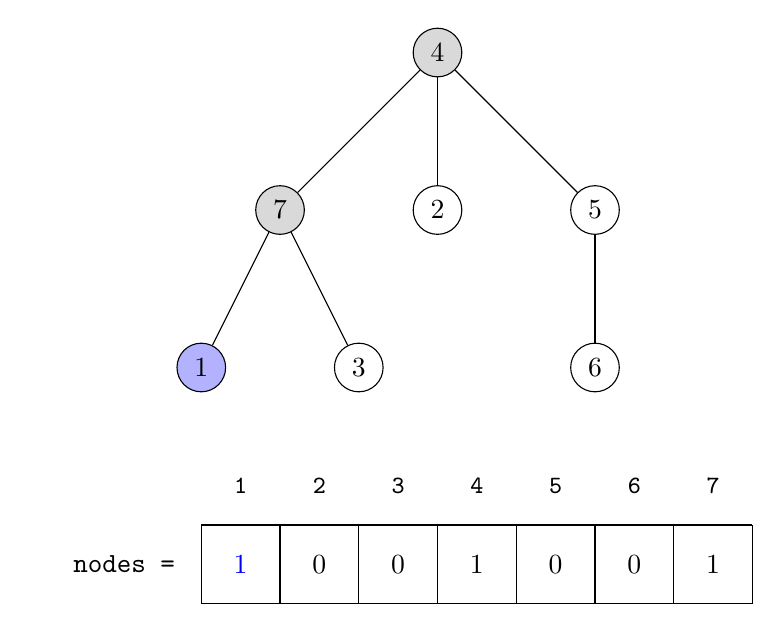
\begin{tikzpicture}

        \begin{scope}{shift={(3,0)}}
            \node[opacity=0] (X) at (-1, 0) { $1$ };

            \node[fill=gray!30,circle,draw] (D) at (4, 5) { $4$ };
            \node[circle,draw,fill=gray!30] (C) at (2, 3) { $7$ };
            \node[circle,draw,fill=white!30] (E) at (4, 3) { $2$ };
            \node[circle,draw] (F) at (6, 3) { $5$ };
            \node[circle,draw,fill=blue!30] (A) at (1, 1) { $1$ };
            \node[circle,draw,fill=white!30] (B) at (3, 1) { $3$ };
            \node[circle,draw,fill=white!30] (G) at (6, 1) { $6$ };

            \draw (A) -- (C);
            \draw (B) -- (C);
            \draw (C) -- (D);
            \draw (D) -- (E);
            \draw (D) -- (F);
            \draw (F) -- (G);

            \node[anchor=west] at (-0.75, -1.5) { \texttt{nodes = } };
            \draw (1, -2) grid (8, -1);

            \node at (1.5, -0.5) { \small \texttt{1} };
            \node at (2.5, -0.5) { \small \texttt{2} };
            \node at (3.5, -0.5) { \small \texttt{3} };
            \node at (4.5, -0.5) { \small \texttt{4} };
            \node at (5.5, -0.5) { \small \texttt{5} };
            \node at (6.5, -0.5) { \small \texttt{6} };
            \node at (7.5, -0.5) { \small \texttt{7} };

            \node at (1.5, -1.5) { \textcolor{blue}{$1$} };
            \node at (2.5, -1.5) { $0$ };
            \node at (3.5, -1.5) { $0$ };
            \node at (4.5, -1.5) { $1$ };
            \node at (5.5, -1.5) { $0$ };
            \node at (6.5, -1.5) { $0$ };
            \node at (7.5, -1.5) { $1$ };

        \end{scope}
    \end{tikzpicture}

\end{frame}

\begin{frame}[fragile]{Visualização do algoritmo que computa o número de nós}

    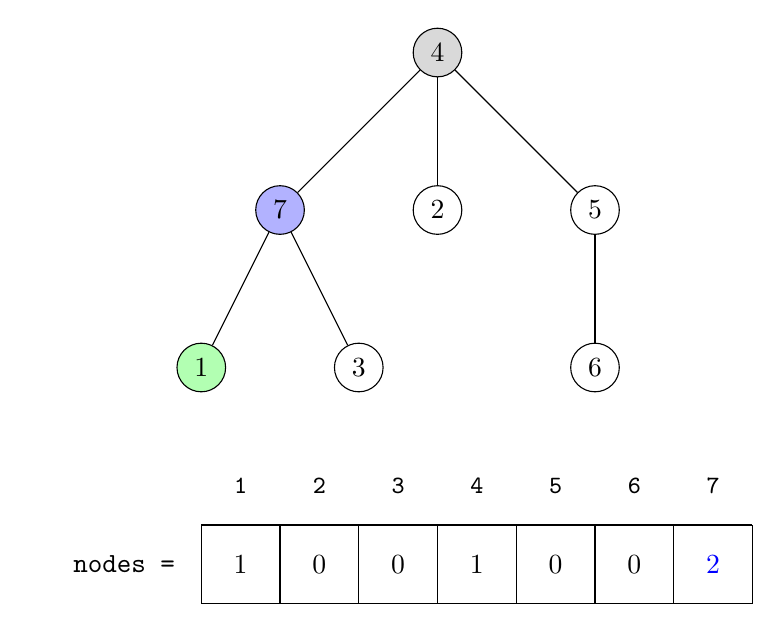
\begin{tikzpicture}

        \begin{scope}{shift={(3,0)}}
            \node[opacity=0] (X) at (-1, 0) { $1$ };

            \node[fill=gray!30,circle,draw] (D) at (4, 5) { $4$ };
            \node[circle,draw,fill=blue!30] (C) at (2, 3) { $7$ };
            \node[circle,draw,fill=white!30] (E) at (4, 3) { $2$ };
            \node[circle,draw] (F) at (6, 3) { $5$ };
            \node[circle,draw,fill=green!30] (A) at (1, 1) { $1$ };
            \node[circle,draw,fill=white!30] (B) at (3, 1) { $3$ };
            \node[circle,draw,fill=white!30] (G) at (6, 1) { $6$ };

            \draw (A) -- (C);
            \draw (B) -- (C);
            \draw (C) -- (D);
            \draw (D) -- (E);
            \draw (D) -- (F);
            \draw (F) -- (G);

            \node[anchor=west] at (-0.75, -1.5) { \texttt{nodes = } };
            \draw (1, -2) grid (8, -1);

            \node at (1.5, -0.5) { \small \texttt{1} };
            \node at (2.5, -0.5) { \small \texttt{2} };
            \node at (3.5, -0.5) { \small \texttt{3} };
            \node at (4.5, -0.5) { \small \texttt{4} };
            \node at (5.5, -0.5) { \small \texttt{5} };
            \node at (6.5, -0.5) { \small \texttt{6} };
            \node at (7.5, -0.5) { \small \texttt{7} };

            \node at (1.5, -1.5) { \textcolor{black}{$1$} };
            \node at (2.5, -1.5) { $0$ };
            \node at (3.5, -1.5) { $0$ };
            \node at (4.5, -1.5) { $1$ };
            \node at (5.5, -1.5) { $0$ };
            \node at (6.5, -1.5) { $0$ };
            \node at (7.5, -1.5) { \textcolor{blue}{$2$} };

        \end{scope}
    \end{tikzpicture}

\end{frame}

\begin{frame}[fragile]{Visualização do algoritmo que computa o número de nós}

    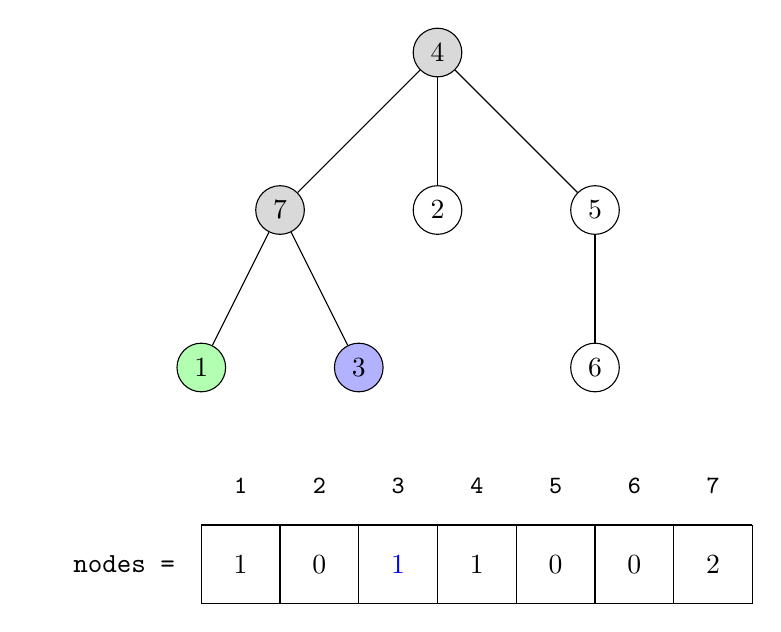
\begin{tikzpicture}

        \begin{scope}{shift={(3,0)}}
            \node[opacity=0] (X) at (-1, 0) { $1$ };

            \node[fill=gray!30,circle,draw] (D) at (4, 5) { $4$ };
            \node[circle,draw,fill=gray!30] (C) at (2, 3) { $7$ };
            \node[circle,draw,fill=white!30] (E) at (4, 3) { $2$ };
            \node[circle,draw] (F) at (6, 3) { $5$ };
            \node[circle,draw,fill=green!30] (A) at (1, 1) { $1$ };
            \node[circle,draw,fill=blue!30] (B) at (3, 1) { $3$ };
            \node[circle,draw,fill=white!30] (G) at (6, 1) { $6$ };

            \draw (A) -- (C);
            \draw (B) -- (C);
            \draw (C) -- (D);
            \draw (D) -- (E);
            \draw (D) -- (F);
            \draw (F) -- (G);

            \node[anchor=west] at (-0.75, -1.5) { \texttt{nodes = } };
            \draw (1, -2) grid (8, -1);

            \node at (1.5, -0.5) { \small \texttt{1} };
            \node at (2.5, -0.5) { \small \texttt{2} };
            \node at (3.5, -0.5) { \small \texttt{3} };
            \node at (4.5, -0.5) { \small \texttt{4} };
            \node at (5.5, -0.5) { \small \texttt{5} };
            \node at (6.5, -0.5) { \small \texttt{6} };
            \node at (7.5, -0.5) { \small \texttt{7} };

            \node at (1.5, -1.5) { \textcolor{black}{$1$} };
            \node at (2.5, -1.5) { $0$ };
            \node at (3.5, -1.5) { \textcolor{blue}{$1$} };
            \node at (4.5, -1.5) { $1$ };
            \node at (5.5, -1.5) { $0$ };
            \node at (6.5, -1.5) { $0$ };
            \node at (7.5, -1.5) { \textcolor{black}{$2$} };

        \end{scope}
    \end{tikzpicture}

\end{frame}

\begin{frame}[fragile]{Visualização do algoritmo que computa o número de nós}

    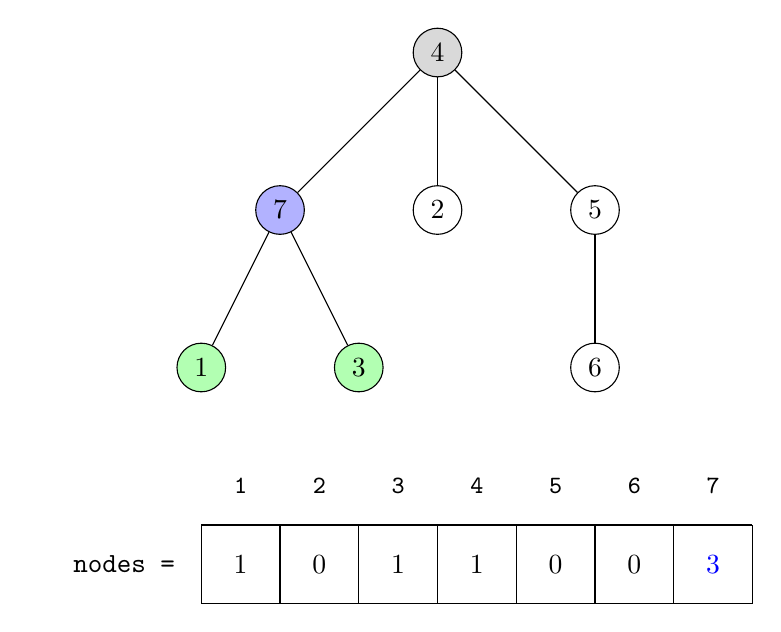
\begin{tikzpicture}

        \begin{scope}{shift={(3,0)}}
            \node[opacity=0] (X) at (-1, 0) { $1$ };

            \node[fill=gray!30,circle,draw] (D) at (4, 5) { $4$ };
            \node[circle,draw,fill=blue!30] (C) at (2, 3) { $7$ };
            \node[circle,draw,fill=white!30] (E) at (4, 3) { $2$ };
            \node[circle,draw] (F) at (6, 3) { $5$ };
            \node[circle,draw,fill=green!30] (A) at (1, 1) { $1$ };
            \node[circle,draw,fill=green!30] (B) at (3, 1) { $3$ };
            \node[circle,draw,fill=white!30] (G) at (6, 1) { $6$ };

            \draw (A) -- (C);
            \draw (B) -- (C);
            \draw (C) -- (D);
            \draw (D) -- (E);
            \draw (D) -- (F);
            \draw (F) -- (G);

            \node[anchor=west] at (-0.75, -1.5) { \texttt{nodes = } };
            \draw (1, -2) grid (8, -1);

            \node at (1.5, -0.5) { \small \texttt{1} };
            \node at (2.5, -0.5) { \small \texttt{2} };
            \node at (3.5, -0.5) { \small \texttt{3} };
            \node at (4.5, -0.5) { \small \texttt{4} };
            \node at (5.5, -0.5) { \small \texttt{5} };
            \node at (6.5, -0.5) { \small \texttt{6} };
            \node at (7.5, -0.5) { \small \texttt{7} };

            \node at (1.5, -1.5) { \textcolor{black}{$1$} };
            \node at (2.5, -1.5) { $0$ };
            \node at (3.5, -1.5) { \textcolor{black}{$1$} };
            \node at (4.5, -1.5) { $1$ };
            \node at (5.5, -1.5) { $0$ };
            \node at (6.5, -1.5) { $0$ };
            \node at (7.5, -1.5) { \textcolor{blue}{$3$} };

        \end{scope}
    \end{tikzpicture}

\end{frame}

\begin{frame}[fragile]{Visualização do algoritmo que computa o número de nós}

    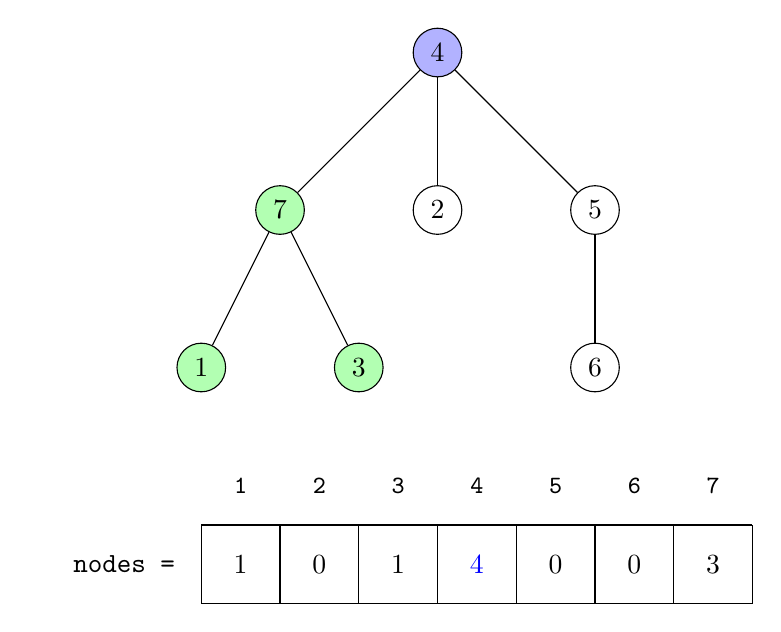
\begin{tikzpicture}

        \begin{scope}{shift={(3,0)}}
            \node[opacity=0] (X) at (-1, 0) { $1$ };

            \node[fill=blue!30,circle,draw] (D) at (4, 5) { $4$ };
            \node[circle,draw,fill=green!30] (C) at (2, 3) { $7$ };
            \node[circle,draw,fill=white!30] (E) at (4, 3) { $2$ };
            \node[circle,draw] (F) at (6, 3) { $5$ };
            \node[circle,draw,fill=green!30] (A) at (1, 1) { $1$ };
            \node[circle,draw,fill=green!30] (B) at (3, 1) { $3$ };
            \node[circle,draw,fill=white!30] (G) at (6, 1) { $6$ };

            \draw (A) -- (C);
            \draw (B) -- (C);
            \draw (C) -- (D);
            \draw (D) -- (E);
            \draw (D) -- (F);
            \draw (F) -- (G);

            \node[anchor=west] at (-0.75, -1.5) { \texttt{nodes = } };
            \draw (1, -2) grid (8, -1);

            \node at (1.5, -0.5) { \small \texttt{1} };
            \node at (2.5, -0.5) { \small \texttt{2} };
            \node at (3.5, -0.5) { \small \texttt{3} };
            \node at (4.5, -0.5) { \small \texttt{4} };
            \node at (5.5, -0.5) { \small \texttt{5} };
            \node at (6.5, -0.5) { \small \texttt{6} };
            \node at (7.5, -0.5) { \small \texttt{7} };

            \node at (1.5, -1.5) { \textcolor{black}{$1$} };
            \node at (2.5, -1.5) { $0$ };
            \node at (3.5, -1.5) { \textcolor{black}{$1$} };
            \node at (4.5, -1.5) { \textcolor{blue}{$4$} };
            \node at (5.5, -1.5) { $0$ };
            \node at (6.5, -1.5) { $0$ };
            \node at (7.5, -1.5) { \textcolor{black}{$3$} };

        \end{scope}
    \end{tikzpicture}

\end{frame}

\begin{frame}[fragile]{Visualização do algoritmo que computa o número de nós}

    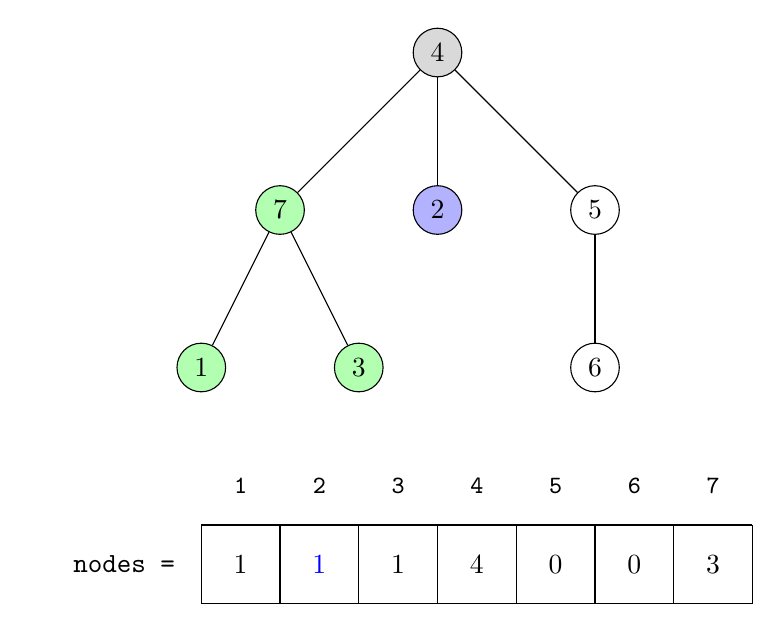
\begin{tikzpicture}

        \begin{scope}{shift={(3,0)}}
            \node[opacity=0] (X) at (-1, 0) { $1$ };

            \node[fill=gray!30,circle,draw] (D) at (4, 5) { $4$ };
            \node[circle,draw,fill=green!30] (C) at (2, 3) { $7$ };
            \node[circle,draw,fill=blue!30] (E) at (4, 3) { $2$ };
            \node[circle,draw] (F) at (6, 3) { $5$ };
            \node[circle,draw,fill=green!30] (A) at (1, 1) { $1$ };
            \node[circle,draw,fill=green!30] (B) at (3, 1) { $3$ };
            \node[circle,draw,fill=white!30] (G) at (6, 1) { $6$ };

            \draw (A) -- (C);
            \draw (B) -- (C);
            \draw (C) -- (D);
            \draw (D) -- (E);
            \draw (D) -- (F);
            \draw (F) -- (G);

            \node[anchor=west] at (-0.75, -1.5) { \texttt{nodes = } };
            \draw (1, -2) grid (8, -1);

            \node at (1.5, -0.5) { \small \texttt{1} };
            \node at (2.5, -0.5) { \small \texttt{2} };
            \node at (3.5, -0.5) { \small \texttt{3} };
            \node at (4.5, -0.5) { \small \texttt{4} };
            \node at (5.5, -0.5) { \small \texttt{5} };
            \node at (6.5, -0.5) { \small \texttt{6} };
            \node at (7.5, -0.5) { \small \texttt{7} };

            \node at (1.5, -1.5) { \textcolor{black}{$1$} };
            \node at (2.5, -1.5) { \textcolor{blue}{$1$} };
            \node at (3.5, -1.5) { \textcolor{black}{$1$} };
            \node at (4.5, -1.5) { \textcolor{black}{$4$} };
            \node at (5.5, -1.5) { $0$ };
            \node at (6.5, -1.5) { $0$ };
            \node at (7.5, -1.5) { \textcolor{black}{$3$} };

        \end{scope}
    \end{tikzpicture}

\end{frame}

\begin{frame}[fragile]{Visualização do algoritmo que computa o número de nós}

    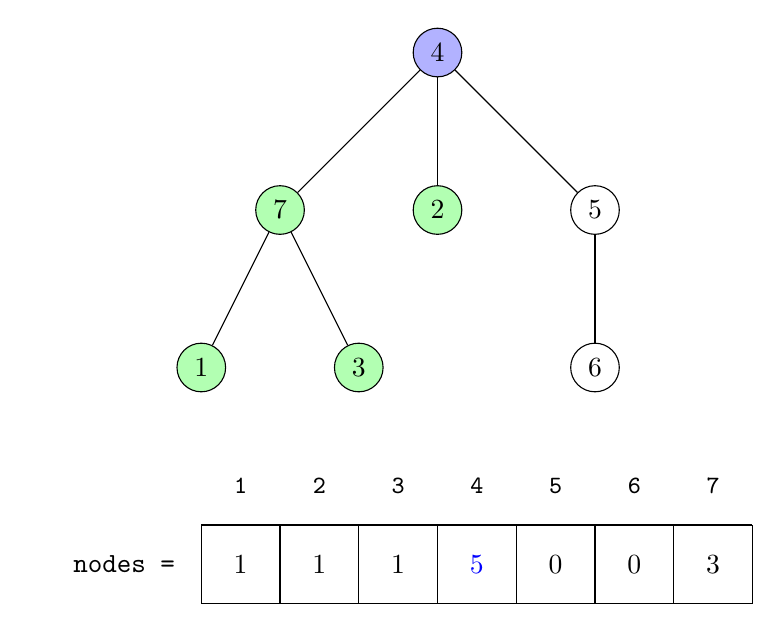
\begin{tikzpicture}

        \begin{scope}{shift={(3,0)}}
            \node[opacity=0] (X) at (-1, 0) { $1$ };

            \node[fill=blue!30,circle,draw] (D) at (4, 5) { $4$ };
            \node[circle,draw,fill=green!30] (C) at (2, 3) { $7$ };
            \node[circle,draw,fill=green!30] (E) at (4, 3) { $2$ };
            \node[circle,draw] (F) at (6, 3) { $5$ };
            \node[circle,draw,fill=green!30] (A) at (1, 1) { $1$ };
            \node[circle,draw,fill=green!30] (B) at (3, 1) { $3$ };
            \node[circle,draw,fill=white!30] (G) at (6, 1) { $6$ };

            \draw (A) -- (C);
            \draw (B) -- (C);
            \draw (C) -- (D);
            \draw (D) -- (E);
            \draw (D) -- (F);
            \draw (F) -- (G);

            \node[anchor=west] at (-0.75, -1.5) { \texttt{nodes = } };
            \draw (1, -2) grid (8, -1);

            \node at (1.5, -0.5) { \small \texttt{1} };
            \node at (2.5, -0.5) { \small \texttt{2} };
            \node at (3.5, -0.5) { \small \texttt{3} };
            \node at (4.5, -0.5) { \small \texttt{4} };
            \node at (5.5, -0.5) { \small \texttt{5} };
            \node at (6.5, -0.5) { \small \texttt{6} };
            \node at (7.5, -0.5) { \small \texttt{7} };

            \node at (1.5, -1.5) { \textcolor{black}{$1$} };
            \node at (2.5, -1.5) { \textcolor{black}{$1$} };
            \node at (3.5, -1.5) { \textcolor{black}{$1$} };
            \node at (4.5, -1.5) { \textcolor{blue}{$5$} };
            \node at (5.5, -1.5) { $0$ };
            \node at (6.5, -1.5) { $0$ };
            \node at (7.5, -1.5) { \textcolor{black}{$3$} };

        \end{scope}
    \end{tikzpicture}

\end{frame}

\begin{frame}[fragile]{Visualização do algoritmo que computa o número de nós}

    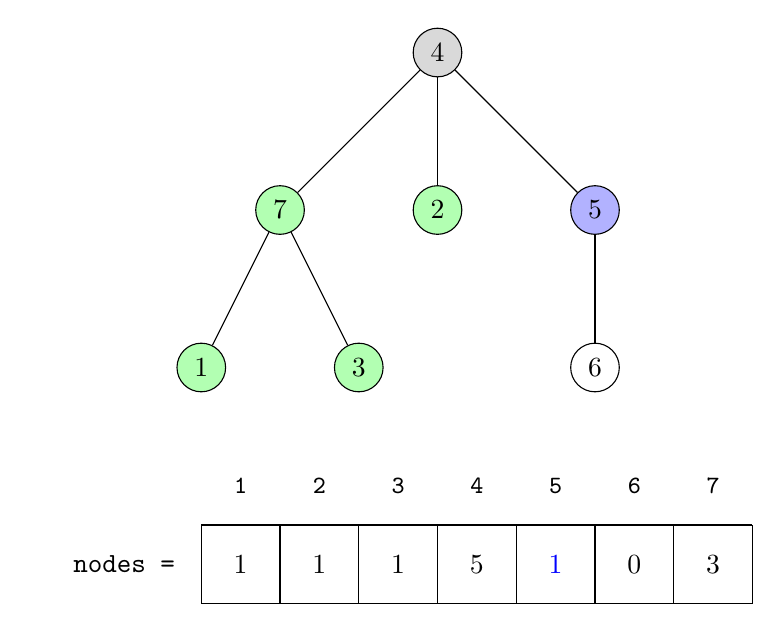
\begin{tikzpicture}

        \begin{scope}{shift={(3,0)}}
            \node[opacity=0] (X) at (-1, 0) { $1$ };

            \node[fill=gray!30,circle,draw] (D) at (4, 5) { $4$ };
            \node[circle,draw,fill=green!30] (C) at (2, 3) { $7$ };
            \node[circle,draw,fill=green!30] (E) at (4, 3) { $2$ };
            \node[circle,draw,fill=blue!30] (F) at (6, 3) { $5$ };
            \node[circle,draw,fill=green!30] (A) at (1, 1) { $1$ };
            \node[circle,draw,fill=green!30] (B) at (3, 1) { $3$ };
            \node[circle,draw,fill=white!30] (G) at (6, 1) { $6$ };

            \draw (A) -- (C);
            \draw (B) -- (C);
            \draw (C) -- (D);
            \draw (D) -- (E);
            \draw (D) -- (F);
            \draw (F) -- (G);

            \node[anchor=west] at (-0.75, -1.5) { \texttt{nodes = } };
            \draw (1, -2) grid (8, -1);

            \node at (1.5, -0.5) { \small \texttt{1} };
            \node at (2.5, -0.5) { \small \texttt{2} };
            \node at (3.5, -0.5) { \small \texttt{3} };
            \node at (4.5, -0.5) { \small \texttt{4} };
            \node at (5.5, -0.5) { \small \texttt{5} };
            \node at (6.5, -0.5) { \small \texttt{6} };
            \node at (7.5, -0.5) { \small \texttt{7} };

            \node at (1.5, -1.5) { \textcolor{black}{$1$} };
            \node at (2.5, -1.5) { \textcolor{black}{$1$} };
            \node at (3.5, -1.5) { \textcolor{black}{$1$} };
            \node at (4.5, -1.5) { \textcolor{black}{$5$} };
            \node at (5.5, -1.5) { \textcolor{blue}{$1$} };
            \node at (6.5, -1.5) { $0$ };
            \node at (7.5, -1.5) { \textcolor{black}{$3$} };

        \end{scope}
    \end{tikzpicture}

\end{frame}

\begin{frame}[fragile]{Visualização do algoritmo que computa o número de nós}

    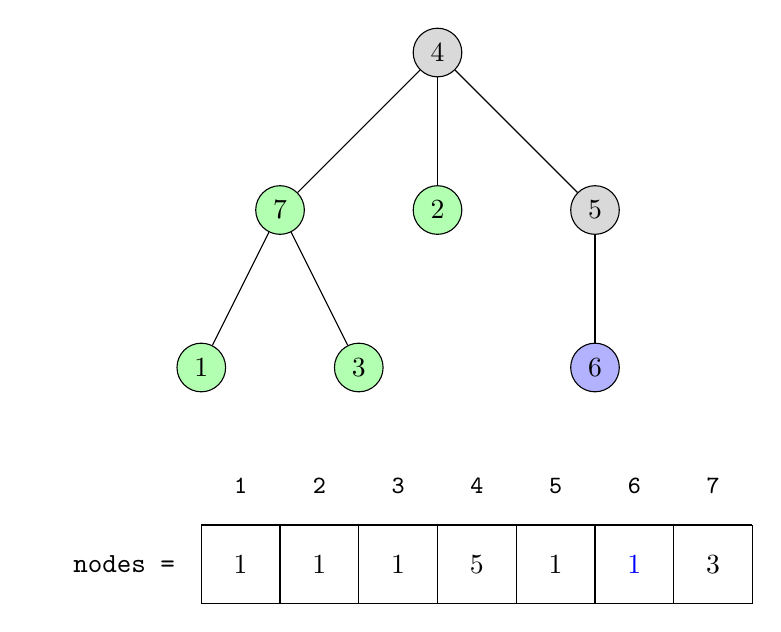
\begin{tikzpicture}

        \begin{scope}{shift={(3,0)}}
            \node[opacity=0] (X) at (-1, 0) { $1$ };

            \node[fill=gray!30,circle,draw] (D) at (4, 5) { $4$ };
            \node[circle,draw,fill=green!30] (C) at (2, 3) { $7$ };
            \node[circle,draw,fill=green!30] (E) at (4, 3) { $2$ };
            \node[circle,draw,fill=gray!30] (F) at (6, 3) { $5$ };
            \node[circle,draw,fill=green!30] (A) at (1, 1) { $1$ };
            \node[circle,draw,fill=green!30] (B) at (3, 1) { $3$ };
            \node[circle,draw,fill=blue!30] (G) at (6, 1) { $6$ };

            \draw (A) -- (C);
            \draw (B) -- (C);
            \draw (C) -- (D);
            \draw (D) -- (E);
            \draw (D) -- (F);
            \draw (F) -- (G);

            \node[anchor=west] at (-0.75, -1.5) { \texttt{nodes = } };
            \draw (1, -2) grid (8, -1);

            \node at (1.5, -0.5) { \small \texttt{1} };
            \node at (2.5, -0.5) { \small \texttt{2} };
            \node at (3.5, -0.5) { \small \texttt{3} };
            \node at (4.5, -0.5) { \small \texttt{4} };
            \node at (5.5, -0.5) { \small \texttt{5} };
            \node at (6.5, -0.5) { \small \texttt{6} };
            \node at (7.5, -0.5) { \small \texttt{7} };

            \node at (1.5, -1.5) { \textcolor{black}{$1$} };
            \node at (2.5, -1.5) { \textcolor{black}{$1$} };
            \node at (3.5, -1.5) { \textcolor{black}{$1$} };
            \node at (4.5, -1.5) { \textcolor{black}{$5$} };
            \node at (5.5, -1.5) { $1$ };
            \node at (6.5, -1.5) { \textcolor{blue}{$1$} };
            \node at (7.5, -1.5) { \textcolor{black}{$3$} };

        \end{scope}
    \end{tikzpicture}

\end{frame}

\begin{frame}[fragile]{Visualização do algoritmo que computa o número de nós}

    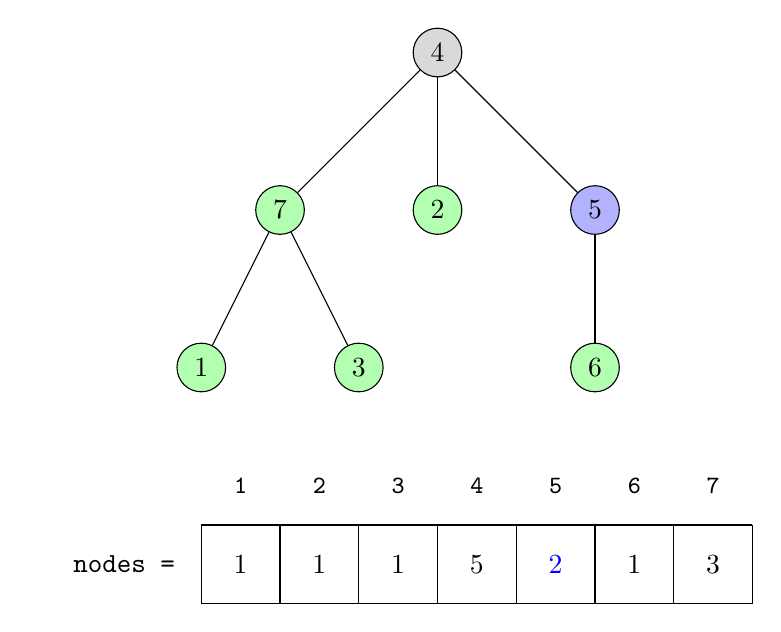
\begin{tikzpicture}

        \begin{scope}{shift={(3,0)}}
            \node[opacity=0] (X) at (-1, 0) { $1$ };

            \node[fill=gray!30,circle,draw] (D) at (4, 5) { $4$ };
            \node[circle,draw,fill=green!30] (C) at (2, 3) { $7$ };
            \node[circle,draw,fill=green!30] (E) at (4, 3) { $2$ };
            \node[circle,draw,fill=blue!30] (F) at (6, 3) { $5$ };
            \node[circle,draw,fill=green!30] (A) at (1, 1) { $1$ };
            \node[circle,draw,fill=green!30] (B) at (3, 1) { $3$ };
            \node[circle,draw,fill=green!30] (G) at (6, 1) { $6$ };

            \draw (A) -- (C);
            \draw (B) -- (C);
            \draw (C) -- (D);
            \draw (D) -- (E);
            \draw (D) -- (F);
            \draw (F) -- (G);

            \node[anchor=west] at (-0.75, -1.5) { \texttt{nodes = } };
            \draw (1, -2) grid (8, -1);

            \node at (1.5, -0.5) { \small \texttt{1} };
            \node at (2.5, -0.5) { \small \texttt{2} };
            \node at (3.5, -0.5) { \small \texttt{3} };
            \node at (4.5, -0.5) { \small \texttt{4} };
            \node at (5.5, -0.5) { \small \texttt{5} };
            \node at (6.5, -0.5) { \small \texttt{6} };
            \node at (7.5, -0.5) { \small \texttt{7} };

            \node at (1.5, -1.5) { \textcolor{black}{$1$} };
            \node at (2.5, -1.5) { \textcolor{black}{$1$} };
            \node at (3.5, -1.5) { \textcolor{black}{$1$} };
            \node at (4.5, -1.5) { \textcolor{black}{$5$} };
            \node at (5.5, -1.5) { \textcolor{blue}{$2$} };
            \node at (6.5, -1.5) { \textcolor{black}{$1$} };
            \node at (7.5, -1.5) { \textcolor{black}{$3$} };

        \end{scope}
    \end{tikzpicture}

\end{frame}

\begin{frame}[fragile]{Visualização do algoritmo que computa o número de nós}

    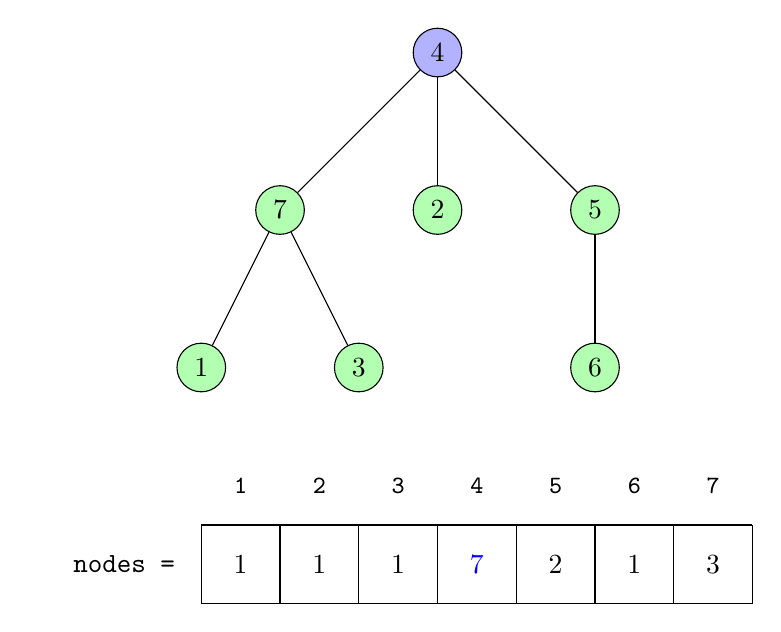
\begin{tikzpicture}

        \begin{scope}{shift={(3,0)}}
            \node[opacity=0] (X) at (-1, 0) { $1$ };

            \node[fill=blue!30,circle,draw] (D) at (4, 5) { $4$ };
            \node[circle,draw,fill=green!30] (C) at (2, 3) { $7$ };
            \node[circle,draw,fill=green!30] (E) at (4, 3) { $2$ };
            \node[circle,draw,fill=green!30] (F) at (6, 3) { $5$ };
            \node[circle,draw,fill=green!30] (A) at (1, 1) { $1$ };
            \node[circle,draw,fill=green!30] (B) at (3, 1) { $3$ };
            \node[circle,draw,fill=green!30] (G) at (6, 1) { $6$ };

            \draw (A) -- (C);
            \draw (B) -- (C);
            \draw (C) -- (D);
            \draw (D) -- (E);
            \draw (D) -- (F);
            \draw (F) -- (G);

            \node[anchor=west] at (-0.75, -1.5) { \texttt{nodes = } };
            \draw (1, -2) grid (8, -1);

            \node at (1.5, -0.5) { \small \texttt{1} };
            \node at (2.5, -0.5) { \small \texttt{2} };
            \node at (3.5, -0.5) { \small \texttt{3} };
            \node at (4.5, -0.5) { \small \texttt{4} };
            \node at (5.5, -0.5) { \small \texttt{5} };
            \node at (6.5, -0.5) { \small \texttt{6} };
            \node at (7.5, -0.5) { \small \texttt{7} };

            \node at (1.5, -1.5) { \textcolor{black}{$1$} };
            \node at (2.5, -1.5) { \textcolor{black}{$1$} };
            \node at (3.5, -1.5) { \textcolor{black}{$1$} };
            \node at (4.5, -1.5) { \textcolor{blue}{$7$} };
            \node at (5.5, -1.5) { \textcolor{black}{$2$} };
            \node at (6.5, -1.5) { \textcolor{black}{$1$} };
            \node at (7.5, -1.5) { \textcolor{black}{$3$} };

        \end{scope}
    \end{tikzpicture}

\end{frame}

\begin{frame}[fragile]{Visualização do algoritmo que computa o número de nós}

    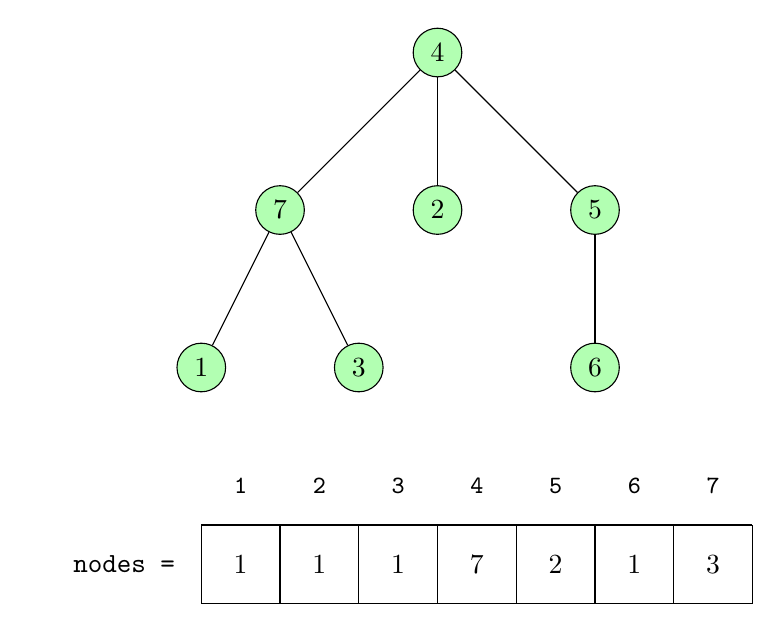
\begin{tikzpicture}

        \begin{scope}{shift={(3,0)}}
            \node[opacity=0] (X) at (-1, 0) { $1$ };

            \node[fill=green!30,circle,draw] (D) at (4, 5) { $4$ };
            \node[circle,draw,fill=green!30] (C) at (2, 3) { $7$ };
            \node[circle,draw,fill=green!30] (E) at (4, 3) { $2$ };
            \node[circle,draw,fill=green!30] (F) at (6, 3) { $5$ };
            \node[circle,draw,fill=green!30] (A) at (1, 1) { $1$ };
            \node[circle,draw,fill=green!30] (B) at (3, 1) { $3$ };
            \node[circle,draw,fill=green!30] (G) at (6, 1) { $6$ };

            \draw (A) -- (C);
            \draw (B) -- (C);
            \draw (C) -- (D);
            \draw (D) -- (E);
            \draw (D) -- (F);
            \draw (F) -- (G);

            \node[anchor=west] at (-0.75, -1.5) { \texttt{nodes = } };
            \draw (1, -2) grid (8, -1);

            \node at (1.5, -0.5) { \small \texttt{1} };
            \node at (2.5, -0.5) { \small \texttt{2} };
            \node at (3.5, -0.5) { \small \texttt{3} };
            \node at (4.5, -0.5) { \small \texttt{4} };
            \node at (5.5, -0.5) { \small \texttt{5} };
            \node at (6.5, -0.5) { \small \texttt{6} };
            \node at (7.5, -0.5) { \small \texttt{7} };

            \node at (1.5, -1.5) { \textcolor{black}{$1$} };
            \node at (2.5, -1.5) { \textcolor{black}{$1$} };
            \node at (3.5, -1.5) { \textcolor{black}{$1$} };
            \node at (4.5, -1.5) { \textcolor{black}{$7$} };
            \node at (5.5, -1.5) { \textcolor{black}{$2$} };
            \node at (6.5, -1.5) { \textcolor{black}{$1$} };
            \node at (7.5, -1.5) { \textcolor{black}{$3$} };

        \end{scope}
    \end{tikzpicture}

\end{frame}


\begin{frame}[fragile]{Implementação da rotina que computa \code{c}{nodes[u]}}
    \inputsnippet{c++}{1}{21}{nodes.cpp}
\end{frame}

\begin{frame}[fragile]{Implementação da rotina que computa \code{c}{nodes[u]}}
    \inputsnippet{c++}{22}{42}{nodes.cpp}
\end{frame}

\begin{frame}[fragile]{Maior caminho até uma folha}

    \begin{itemize}
        \item Outro exemplo de DFS com DP é o cálculo do tamanho (em número de arestas) do
            maior caminho  \code{c}{to_leaf[u]} de $u$ até uma folha

        \item Se $u$ for uma folha então \code{c}{to_leaf[u]} = 0

        \item Caso contrário, \code{c}{to_leaf[u]} = 1 + $\max \lbrace$ \code{c}{to_leaf}[$v_i$] 
        $\rbrace$, onde $v_i$ são os filhos de $u$

        \item Esta rotina pode ser facilmente adaptada para retornar o tamanho como a soma dos
            pesos das arestas
    \end{itemize}

\end{frame}

\begin{frame}[fragile]{Visualização do algoritmo que computa \texttt{to\_leaf}}

    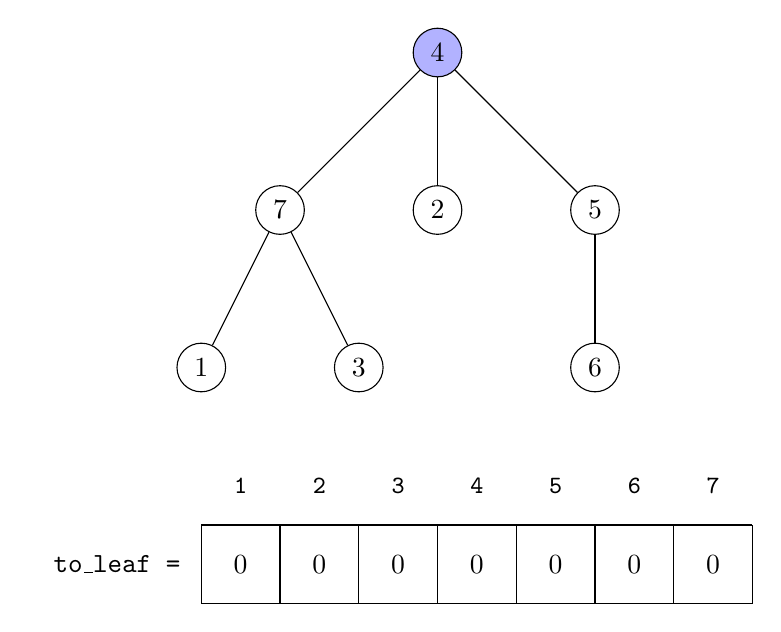
\begin{tikzpicture}

        \begin{scope}{shift={(3,0)}}
            \node[opacity=0] (X) at (-1, 0) { $1$ };

            \node[fill=blue!30,circle,draw] (D) at (4, 5) { $4$ };
            \node[circle,draw] (C) at (2, 3) { $7$ };
            \node[circle,draw,fill=white!30] (E) at (4, 3) { $2$ };
            \node[circle,draw] (F) at (6, 3) { $5$ };
            \node[circle,draw,fill=white!30] (A) at (1, 1) { $1$ };
            \node[circle,draw,fill=white!30] (B) at (3, 1) { $3$ };
            \node[circle,draw,fill=white!30] (G) at (6, 1) { $6$ };

            \draw (A) -- (C);
            \draw (B) -- (C);
            \draw (C) -- (D);
            \draw (D) -- (E);
            \draw (D) -- (F);
            \draw (F) -- (G);

            \node[anchor=west] at (-1.0, -1.5) { \texttt{to\_leaf = } };
            \draw (1, -2) grid (8, -1);

            \node at (1.5, -0.5) { \small \texttt{1} };
            \node at (2.5, -0.5) { \small \texttt{2} };
            \node at (3.5, -0.5) { \small \texttt{3} };
            \node at (4.5, -0.5) { \small \texttt{4} };
            \node at (5.5, -0.5) { \small \texttt{5} };
            \node at (6.5, -0.5) { \small \texttt{6} };
            \node at (7.5, -0.5) { \small \texttt{7} };

            \node at (1.5, -1.5) { $0$ };
            \node at (2.5, -1.5) { $0$ };
            \node at (3.5, -1.5) { $0$ };
            \node at (4.5, -1.5) { \textcolor{black}{$0$} };
            \node at (5.5, -1.5) { $0$ };
            \node at (6.5, -1.5) { $0$ };
            \node at (7.5, -1.5) { $0$ };

        \end{scope}
    \end{tikzpicture}

\end{frame}

\begin{frame}[fragile]{Visualização do algoritmo que computa \texttt{to\_leaf}}

    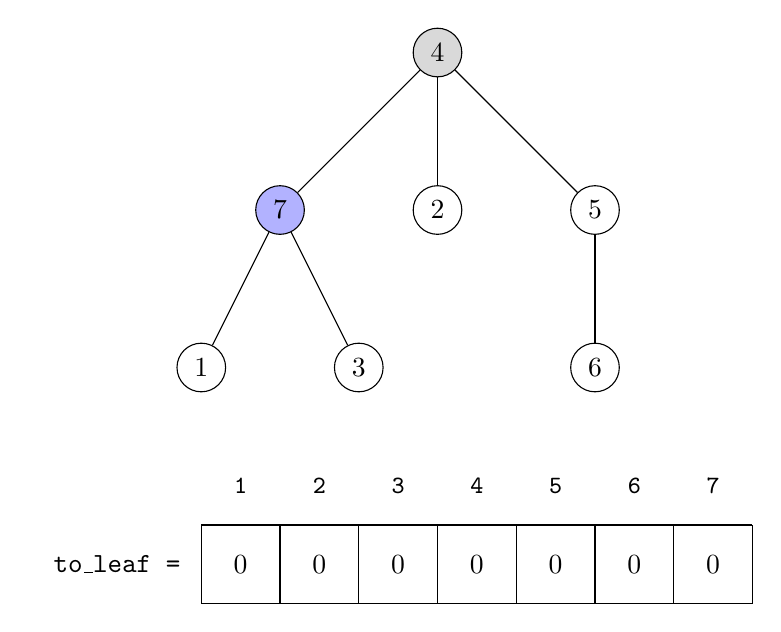
\begin{tikzpicture}

        \begin{scope}{shift={(3,0)}}
            \node[opacity=0] (X) at (-1, 0) { $1$ };

            \node[fill=gray!30,circle,draw] (D) at (4, 5) { $4$ };
            \node[circle,draw,fill=blue!30] (C) at (2, 3) { $7$ };
            \node[circle,draw,fill=white!30] (E) at (4, 3) { $2$ };
            \node[circle,draw] (F) at (6, 3) { $5$ };
            \node[circle,draw,fill=white!30] (A) at (1, 1) { $1$ };
            \node[circle,draw,fill=white!30] (B) at (3, 1) { $3$ };
            \node[circle,draw,fill=white!30] (G) at (6, 1) { $6$ };

            \draw (A) -- (C);
            \draw (B) -- (C);
            \draw (C) -- (D);
            \draw (D) -- (E);
            \draw (D) -- (F);
            \draw (F) -- (G);

            \node[anchor=west] at (-1.0, -1.5) { \texttt{to\_leaf = } };
            \draw (1, -2) grid (8, -1);

            \node at (1.5, -0.5) { \small \texttt{1} };
            \node at (2.5, -0.5) { \small \texttt{2} };
            \node at (3.5, -0.5) { \small \texttt{3} };
            \node at (4.5, -0.5) { \small \texttt{4} };
            \node at (5.5, -0.5) { \small \texttt{5} };
            \node at (6.5, -0.5) { \small \texttt{6} };
            \node at (7.5, -0.5) { \small \texttt{7} };

            \node at (1.5, -1.5) { $0$ };
            \node at (2.5, -1.5) { $0$ };
            \node at (3.5, -1.5) { $0$ };
            \node at (4.5, -1.5) { \textcolor{black}{$0$} };
            \node at (5.5, -1.5) { $0$ };
            \node at (6.5, -1.5) { $0$ };
            \node at (7.5, -1.5) { $0$ };

        \end{scope}
    \end{tikzpicture}

\end{frame}

\begin{frame}[fragile]{Visualização do algoritmo que computa \texttt{to\_leaf}}

    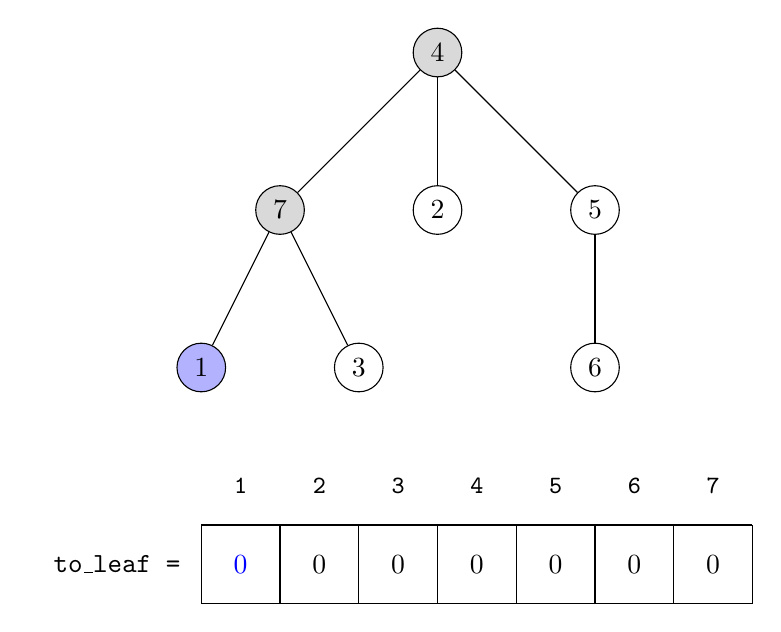
\begin{tikzpicture}

        \begin{scope}{shift={(3,0)}}
            \node[opacity=0] (X) at (-1, 0) { $1$ };

            \node[fill=gray!30,circle,draw] (D) at (4, 5) { $4$ };
            \node[circle,draw,fill=gray!30] (C) at (2, 3) { $7$ };
            \node[circle,draw,fill=white!30] (E) at (4, 3) { $2$ };
            \node[circle,draw] (F) at (6, 3) { $5$ };
            \node[circle,draw,fill=blue!30] (A) at (1, 1) { $1$ };
            \node[circle,draw,fill=white!30] (B) at (3, 1) { $3$ };
            \node[circle,draw,fill=white!30] (G) at (6, 1) { $6$ };

            \draw (A) -- (C);
            \draw (B) -- (C);
            \draw (C) -- (D);
            \draw (D) -- (E);
            \draw (D) -- (F);
            \draw (F) -- (G);

            \node[anchor=west] at (-1.0, -1.5) { \texttt{to\_leaf = } };
            \draw (1, -2) grid (8, -1);

            \node at (1.5, -0.5) { \small \texttt{1} };
            \node at (2.5, -0.5) { \small \texttt{2} };
            \node at (3.5, -0.5) { \small \texttt{3} };
            \node at (4.5, -0.5) { \small \texttt{4} };
            \node at (5.5, -0.5) { \small \texttt{5} };
            \node at (6.5, -0.5) { \small \texttt{6} };
            \node at (7.5, -0.5) { \small \texttt{7} };

            \node at (1.5, -1.5) { \textcolor{blue}{$0$} };
            \node at (2.5, -1.5) { $0$ };
            \node at (3.5, -1.5) { $0$ };
            \node at (4.5, -1.5) { \textcolor{black}{$0$} };
            \node at (5.5, -1.5) { $0$ };
            \node at (6.5, -1.5) { $0$ };
            \node at (7.5, -1.5) { $0$ };

        \end{scope}
    \end{tikzpicture}

\end{frame}

\begin{frame}[fragile]{Visualização do algoritmo que computa \texttt{to\_leaf}}

    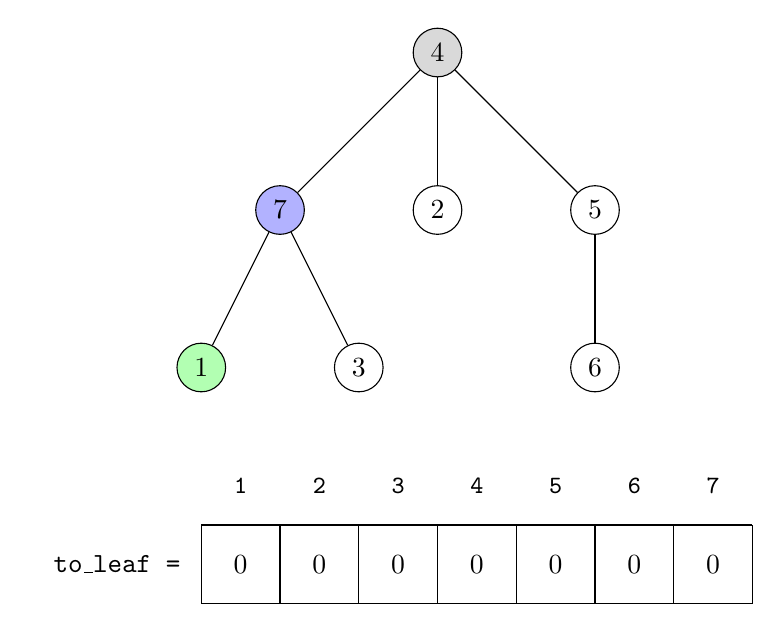
\begin{tikzpicture}

        \begin{scope}{shift={(3,0)}}
            \node[opacity=0] (X) at (-1, 0) { $1$ };

            \node[fill=gray!30,circle,draw] (D) at (4, 5) { $4$ };
            \node[circle,draw,fill=blue!30] (C) at (2, 3) { $7$ };
            \node[circle,draw,fill=white!30] (E) at (4, 3) { $2$ };
            \node[circle,draw] (F) at (6, 3) { $5$ };
            \node[circle,draw,fill=green!30] (A) at (1, 1) { $1$ };
            \node[circle,draw,fill=white!30] (B) at (3, 1) { $3$ };
            \node[circle,draw,fill=white!30] (G) at (6, 1) { $6$ };

            \draw (A) -- (C);
            \draw (B) -- (C);
            \draw (C) -- (D);
            \draw (D) -- (E);
            \draw (D) -- (F);
            \draw (F) -- (G);

            \node[anchor=west] at (-1.0, -1.5) { \texttt{to\_leaf = } };
            \draw (1, -2) grid (8, -1);

            \node at (1.5, -0.5) { \small \texttt{1} };
            \node at (2.5, -0.5) { \small \texttt{2} };
            \node at (3.5, -0.5) { \small \texttt{3} };
            \node at (4.5, -0.5) { \small \texttt{4} };
            \node at (5.5, -0.5) { \small \texttt{5} };
            \node at (6.5, -0.5) { \small \texttt{6} };
            \node at (7.5, -0.5) { \small \texttt{7} };

            \node at (1.5, -1.5) { \textcolor{black}{$0$} };
            \node at (2.5, -1.5) { $0$ };
            \node at (3.5, -1.5) { $0$ };
            \node at (4.5, -1.5) { \textcolor{black}{$0$} };
            \node at (5.5, -1.5) { $0$ };
            \node at (6.5, -1.5) { $0$ };
            \node at (7.5, -1.5) { $0$ };

        \end{scope}
    \end{tikzpicture}

\end{frame}

\begin{frame}[fragile]{Visualização do algoritmo que computa \texttt{to\_leaf}}

    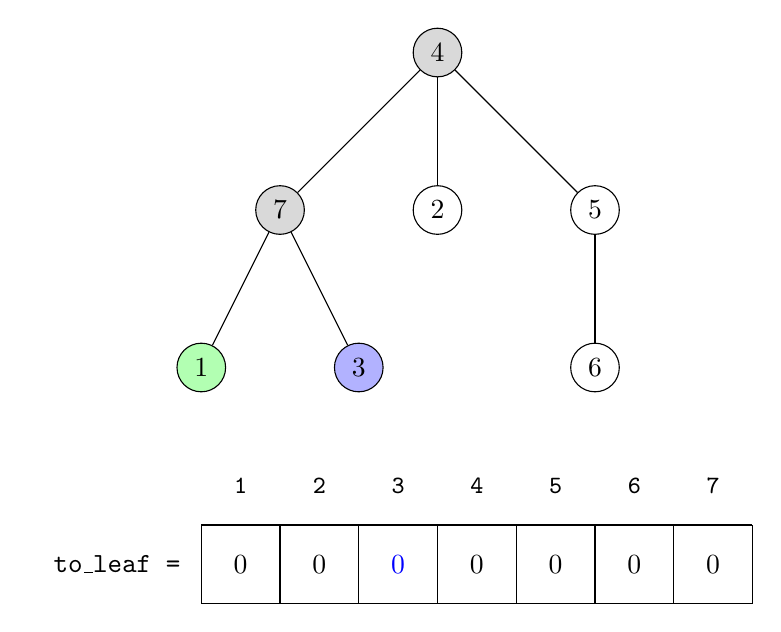
\begin{tikzpicture}

        \begin{scope}{shift={(3,0)}}
            \node[opacity=0] (X) at (-1, 0) { $1$ };

            \node[fill=gray!30,circle,draw] (D) at (4, 5) { $4$ };
            \node[circle,draw,fill=gray!30] (C) at (2, 3) { $7$ };
            \node[circle,draw,fill=white!30] (E) at (4, 3) { $2$ };
            \node[circle,draw] (F) at (6, 3) { $5$ };
            \node[circle,draw,fill=green!30] (A) at (1, 1) { $1$ };
            \node[circle,draw,fill=blue!30] (B) at (3, 1) { $3$ };
            \node[circle,draw,fill=white!30] (G) at (6, 1) { $6$ };

            \draw (A) -- (C);
            \draw (B) -- (C);
            \draw (C) -- (D);
            \draw (D) -- (E);
            \draw (D) -- (F);
            \draw (F) -- (G);

            \node[anchor=west] at (-1.0, -1.5) { \texttt{to\_leaf = } };
            \draw (1, -2) grid (8, -1);

            \node at (1.5, -0.5) { \small \texttt{1} };
            \node at (2.5, -0.5) { \small \texttt{2} };
            \node at (3.5, -0.5) { \small \texttt{3} };
            \node at (4.5, -0.5) { \small \texttt{4} };
            \node at (5.5, -0.5) { \small \texttt{5} };
            \node at (6.5, -0.5) { \small \texttt{6} };
            \node at (7.5, -0.5) { \small \texttt{7} };

            \node at (1.5, -1.5) { \textcolor{black}{$0$} };
            \node at (2.5, -1.5) { $0$ };
            \node at (3.5, -1.5) { \textcolor{blue}{$0$} };
            \node at (4.5, -1.5) { \textcolor{black}{$0$} };
            \node at (5.5, -1.5) { $0$ };
            \node at (6.5, -1.5) { $0$ };
            \node at (7.5, -1.5) { $0$ };

        \end{scope}
    \end{tikzpicture}

\end{frame}

\begin{frame}[fragile]{Visualização do algoritmo que computa \texttt{to\_leaf}}

    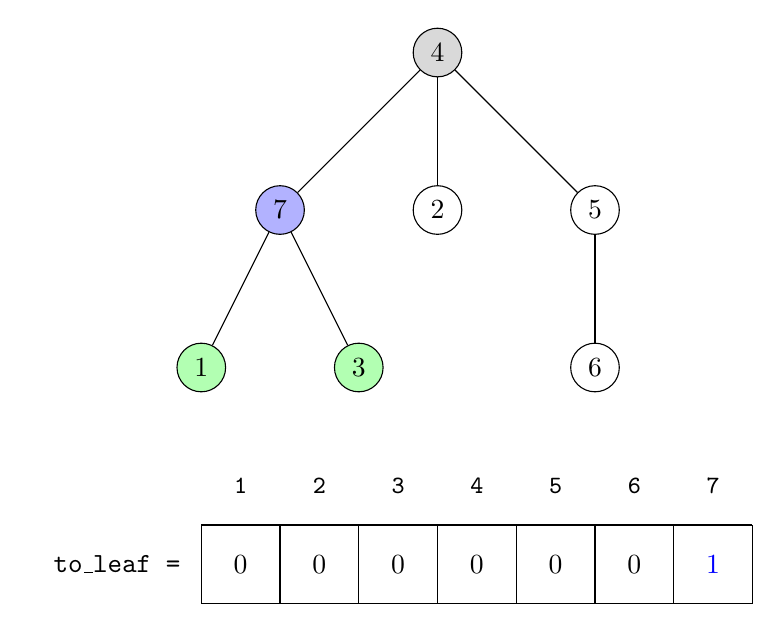
\begin{tikzpicture}

        \begin{scope}{shift={(3,0)}}
            \node[opacity=0] (X) at (-1, 0) { $1$ };

            \node[fill=gray!30,circle,draw] (D) at (4, 5) { $4$ };
            \node[circle,draw,fill=blue!30] (C) at (2, 3) { $7$ };
            \node[circle,draw,fill=white!30] (E) at (4, 3) { $2$ };
            \node[circle,draw] (F) at (6, 3) { $5$ };
            \node[circle,draw,fill=green!30] (A) at (1, 1) { $1$ };
            \node[circle,draw,fill=green!30] (B) at (3, 1) { $3$ };
            \node[circle,draw,fill=white!30] (G) at (6, 1) { $6$ };

            \draw (A) -- (C);
            \draw (B) -- (C);
            \draw (C) -- (D);
            \draw (D) -- (E);
            \draw (D) -- (F);
            \draw (F) -- (G);

            \node[anchor=west] at (-1.0, -1.5) { \texttt{to\_leaf = } };
            \draw (1, -2) grid (8, -1);

            \node at (1.5, -0.5) { \small \texttt{1} };
            \node at (2.5, -0.5) { \small \texttt{2} };
            \node at (3.5, -0.5) { \small \texttt{3} };
            \node at (4.5, -0.5) { \small \texttt{4} };
            \node at (5.5, -0.5) { \small \texttt{5} };
            \node at (6.5, -0.5) { \small \texttt{6} };
            \node at (7.5, -0.5) { \small \texttt{7} };

            \node at (1.5, -1.5) { \textcolor{black}{$0$} };
            \node at (2.5, -1.5) { $0$ };
            \node at (3.5, -1.5) { \textcolor{black}{$0$} };
            \node at (4.5, -1.5) { \textcolor{black}{$0$} };
            \node at (5.5, -1.5) { $0$ };
            \node at (6.5, -1.5) { $0$ };
            \node at (7.5, -1.5) { \textcolor{blue}{$1$} };

        \end{scope}
    \end{tikzpicture}

\end{frame}

\begin{frame}[fragile]{Visualização do algoritmo que computa \texttt{to\_leaf}}

    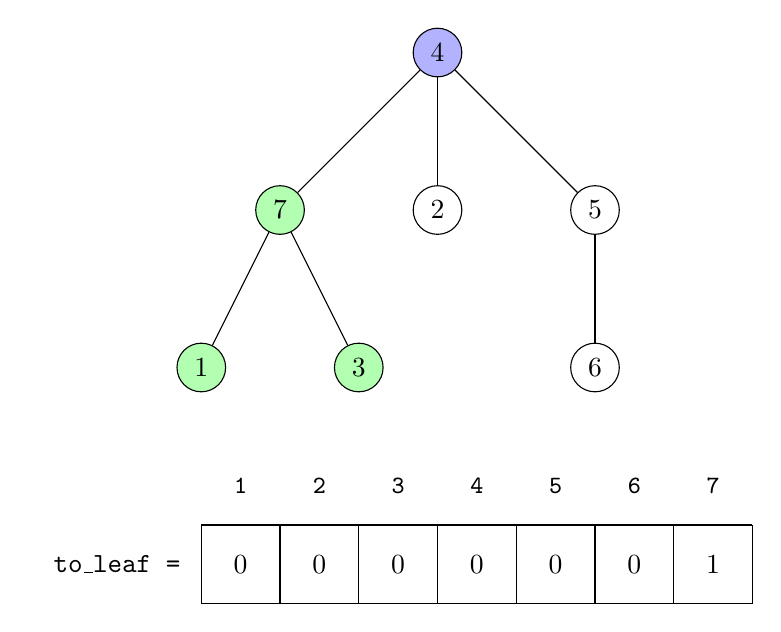
\begin{tikzpicture}

        \begin{scope}{shift={(3,0)}}
            \node[opacity=0] (X) at (-1, 0) { $1$ };

            \node[fill=blue!30,circle,draw] (D) at (4, 5) { $4$ };
            \node[circle,draw,fill=green!30] (C) at (2, 3) { $7$ };
            \node[circle,draw,fill=white!30] (E) at (4, 3) { $2$ };
            \node[circle,draw] (F) at (6, 3) { $5$ };
            \node[circle,draw,fill=green!30] (A) at (1, 1) { $1$ };
            \node[circle,draw,fill=green!30] (B) at (3, 1) { $3$ };
            \node[circle,draw,fill=white!30] (G) at (6, 1) { $6$ };

            \draw (A) -- (C);
            \draw (B) -- (C);
            \draw (C) -- (D);
            \draw (D) -- (E);
            \draw (D) -- (F);
            \draw (F) -- (G);

            \node[anchor=west] at (-1.0, -1.5) { \texttt{to\_leaf = } };
            \draw (1, -2) grid (8, -1);

            \node at (1.5, -0.5) { \small \texttt{1} };
            \node at (2.5, -0.5) { \small \texttt{2} };
            \node at (3.5, -0.5) { \small \texttt{3} };
            \node at (4.5, -0.5) { \small \texttt{4} };
            \node at (5.5, -0.5) { \small \texttt{5} };
            \node at (6.5, -0.5) { \small \texttt{6} };
            \node at (7.5, -0.5) { \small \texttt{7} };

            \node at (1.5, -1.5) { \textcolor{black}{$0$} };
            \node at (2.5, -1.5) { $0$ };
            \node at (3.5, -1.5) { \textcolor{black}{$0$} };
            \node at (4.5, -1.5) { \textcolor{black}{$0$} };
            \node at (5.5, -1.5) { $0$ };
            \node at (6.5, -1.5) { $0$ };
            \node at (7.5, -1.5) { \textcolor{black}{$1$} };

        \end{scope}
    \end{tikzpicture}

\end{frame}

\begin{frame}[fragile]{Visualização do algoritmo que computa \texttt{to\_leaf}}

    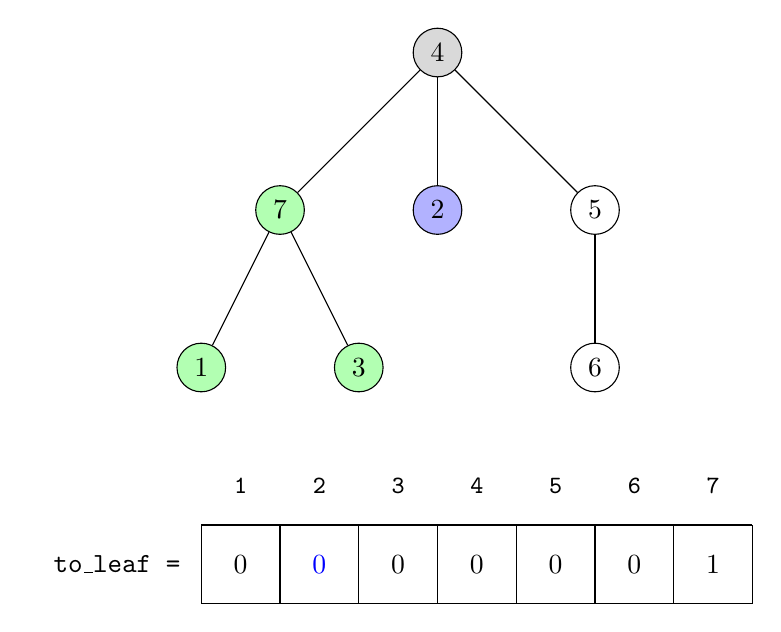
\begin{tikzpicture}

        \begin{scope}{shift={(3,0)}}
            \node[opacity=0] (X) at (-1, 0) { $1$ };

            \node[fill=gray!30,circle,draw] (D) at (4, 5) { $4$ };
            \node[circle,draw,fill=green!30] (C) at (2, 3) { $7$ };
            \node[circle,draw,fill=blue!30] (E) at (4, 3) { $2$ };
            \node[circle,draw] (F) at (6, 3) { $5$ };
            \node[circle,draw,fill=green!30] (A) at (1, 1) { $1$ };
            \node[circle,draw,fill=green!30] (B) at (3, 1) { $3$ };
            \node[circle,draw,fill=white!30] (G) at (6, 1) { $6$ };

            \draw (A) -- (C);
            \draw (B) -- (C);
            \draw (C) -- (D);
            \draw (D) -- (E);
            \draw (D) -- (F);
            \draw (F) -- (G);

            \node[anchor=west] at (-1.0, -1.5) { \texttt{to\_leaf = } };
            \draw (1, -2) grid (8, -1);

            \node at (1.5, -0.5) { \small \texttt{1} };
            \node at (2.5, -0.5) { \small \texttt{2} };
            \node at (3.5, -0.5) { \small \texttt{3} };
            \node at (4.5, -0.5) { \small \texttt{4} };
            \node at (5.5, -0.5) { \small \texttt{5} };
            \node at (6.5, -0.5) { \small \texttt{6} };
            \node at (7.5, -0.5) { \small \texttt{7} };

            \node at (1.5, -1.5) { \textcolor{black}{$0$} };
            \node at (2.5, -1.5) { \textcolor{blue}{$0$} };
            \node at (3.5, -1.5) { \textcolor{black}{$0$} };
            \node at (4.5, -1.5) { \textcolor{black}{$0$} };
            \node at (5.5, -1.5) { $0$ };
            \node at (6.5, -1.5) { $0$ };
            \node at (7.5, -1.5) { \textcolor{black}{$1$} };

        \end{scope}
    \end{tikzpicture}

\end{frame}

\begin{frame}[fragile]{Visualização do algoritmo que computa \texttt{to\_leaf}}

    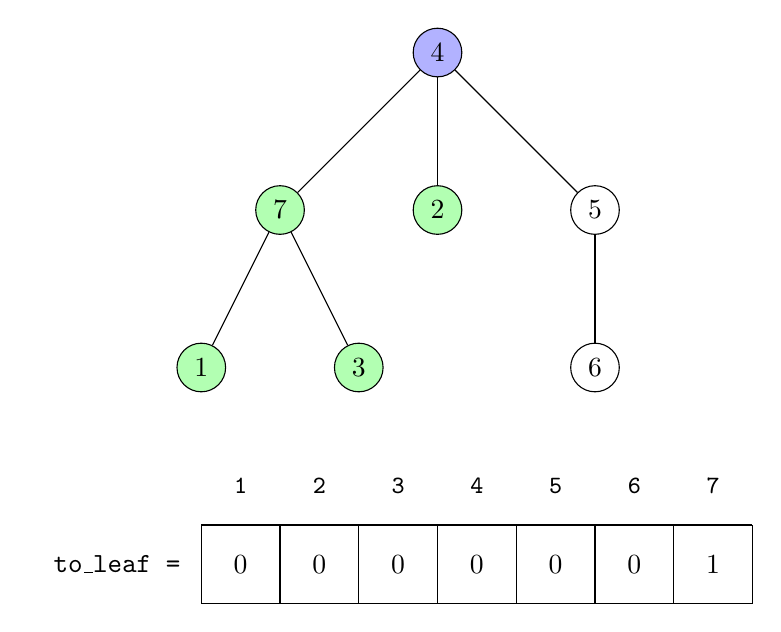
\begin{tikzpicture}

        \begin{scope}{shift={(3,0)}}
            \node[opacity=0] (X) at (-1, 0) { $1$ };

            \node[fill=blue!30,circle,draw] (D) at (4, 5) { $4$ };
            \node[circle,draw,fill=green!30] (C) at (2, 3) { $7$ };
            \node[circle,draw,fill=green!30] (E) at (4, 3) { $2$ };
            \node[circle,draw] (F) at (6, 3) { $5$ };
            \node[circle,draw,fill=green!30] (A) at (1, 1) { $1$ };
            \node[circle,draw,fill=green!30] (B) at (3, 1) { $3$ };
            \node[circle,draw,fill=white!30] (G) at (6, 1) { $6$ };

            \draw (A) -- (C);
            \draw (B) -- (C);
            \draw (C) -- (D);
            \draw (D) -- (E);
            \draw (D) -- (F);
            \draw (F) -- (G);

            \node[anchor=west] at (-1.0, -1.5) { \texttt{to\_leaf = } };
            \draw (1, -2) grid (8, -1);

            \node at (1.5, -0.5) { \small \texttt{1} };
            \node at (2.5, -0.5) { \small \texttt{2} };
            \node at (3.5, -0.5) { \small \texttt{3} };
            \node at (4.5, -0.5) { \small \texttt{4} };
            \node at (5.5, -0.5) { \small \texttt{5} };
            \node at (6.5, -0.5) { \small \texttt{6} };
            \node at (7.5, -0.5) { \small \texttt{7} };

            \node at (1.5, -1.5) { \textcolor{black}{$0$} };
            \node at (2.5, -1.5) { \textcolor{black}{$0$} };
            \node at (3.5, -1.5) { \textcolor{black}{$0$} };
            \node at (4.5, -1.5) { \textcolor{black}{$0$} };
            \node at (5.5, -1.5) { $0$ };
            \node at (6.5, -1.5) { $0$ };
            \node at (7.5, -1.5) { \textcolor{black}{$1$} };

        \end{scope}
    \end{tikzpicture}

\end{frame}

\begin{frame}[fragile]{Visualização do algoritmo que computa \texttt{to\_leaf}}

    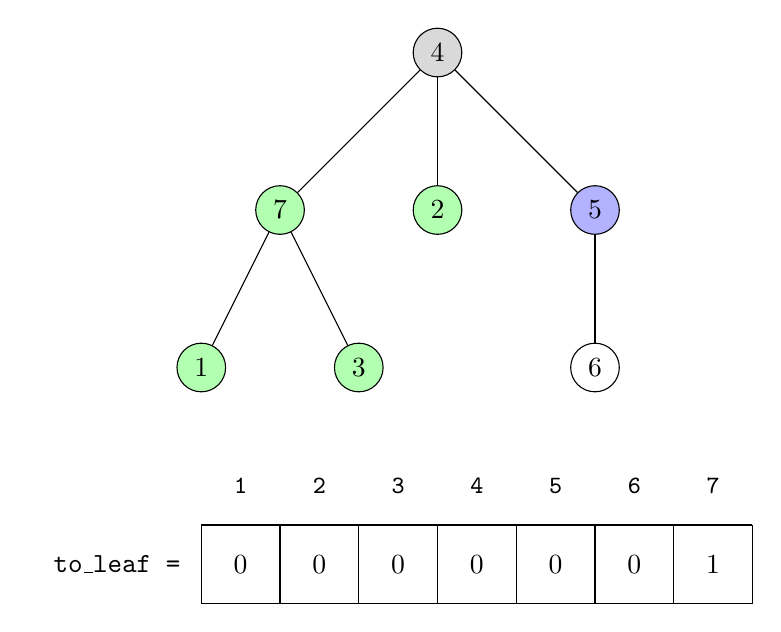
\begin{tikzpicture}

        \begin{scope}{shift={(3,0)}}
            \node[opacity=0] (X) at (-1, 0) { $1$ };

            \node[fill=gray!30,circle,draw] (D) at (4, 5) { $4$ };
            \node[circle,draw,fill=green!30] (C) at (2, 3) { $7$ };
            \node[circle,draw,fill=green!30] (E) at (4, 3) { $2$ };
            \node[circle,draw,fill=blue!30] (F) at (6, 3) { $5$ };
            \node[circle,draw,fill=green!30] (A) at (1, 1) { $1$ };
            \node[circle,draw,fill=green!30] (B) at (3, 1) { $3$ };
            \node[circle,draw,fill=white!30] (G) at (6, 1) { $6$ };

            \draw (A) -- (C);
            \draw (B) -- (C);
            \draw (C) -- (D);
            \draw (D) -- (E);
            \draw (D) -- (F);
            \draw (F) -- (G);

            \node[anchor=west] at (-1.0, -1.5) { \texttt{to\_leaf = } };
            \draw (1, -2) grid (8, -1);

            \node at (1.5, -0.5) { \small \texttt{1} };
            \node at (2.5, -0.5) { \small \texttt{2} };
            \node at (3.5, -0.5) { \small \texttt{3} };
            \node at (4.5, -0.5) { \small \texttt{4} };
            \node at (5.5, -0.5) { \small \texttt{5} };
            \node at (6.5, -0.5) { \small \texttt{6} };
            \node at (7.5, -0.5) { \small \texttt{7} };

            \node at (1.5, -1.5) { \textcolor{black}{$0$} };
            \node at (2.5, -1.5) { \textcolor{black}{$0$} };
            \node at (3.5, -1.5) { \textcolor{black}{$0$} };
            \node at (4.5, -1.5) { \textcolor{black}{$0$} };
            \node at (5.5, -1.5) { $0$ };
            \node at (6.5, -1.5) { $0$ };
            \node at (7.5, -1.5) { \textcolor{black}{$1$} };

        \end{scope}
    \end{tikzpicture}

\end{frame}

\begin{frame}[fragile]{Visualização do algoritmo que computa \texttt{to\_leaf}}

    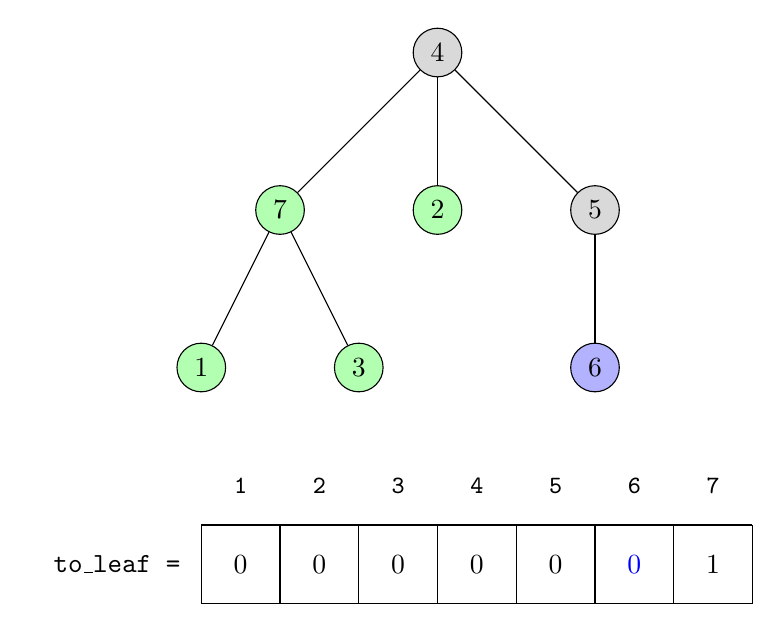
\begin{tikzpicture}

        \begin{scope}{shift={(3,0)}}
            \node[opacity=0] (X) at (-1, 0) { $1$ };

            \node[fill=gray!30,circle,draw] (D) at (4, 5) { $4$ };
            \node[circle,draw,fill=green!30] (C) at (2, 3) { $7$ };
            \node[circle,draw,fill=green!30] (E) at (4, 3) { $2$ };
            \node[circle,draw,fill=gray!30] (F) at (6, 3) { $5$ };
            \node[circle,draw,fill=green!30] (A) at (1, 1) { $1$ };
            \node[circle,draw,fill=green!30] (B) at (3, 1) { $3$ };
            \node[circle,draw,fill=blue!30] (G) at (6, 1) { $6$ };

            \draw (A) -- (C);
            \draw (B) -- (C);
            \draw (C) -- (D);
            \draw (D) -- (E);
            \draw (D) -- (F);
            \draw (F) -- (G);

            \node[anchor=west] at (-1.0, -1.5) { \texttt{to\_leaf = } };
            \draw (1, -2) grid (8, -1);

            \node at (1.5, -0.5) { \small \texttt{1} };
            \node at (2.5, -0.5) { \small \texttt{2} };
            \node at (3.5, -0.5) { \small \texttt{3} };
            \node at (4.5, -0.5) { \small \texttt{4} };
            \node at (5.5, -0.5) { \small \texttt{5} };
            \node at (6.5, -0.5) { \small \texttt{6} };
            \node at (7.5, -0.5) { \small \texttt{7} };

            \node at (1.5, -1.5) { \textcolor{black}{$0$} };
            \node at (2.5, -1.5) { \textcolor{black}{$0$} };
            \node at (3.5, -1.5) { \textcolor{black}{$0$} };
            \node at (4.5, -1.5) { \textcolor{black}{$0$} };
            \node at (5.5, -1.5) { $0$ };
            \node at (6.5, -1.5) { \textcolor{blue}{$0$} };
            \node at (7.5, -1.5) { \textcolor{black}{$1$} };

        \end{scope}
    \end{tikzpicture}

\end{frame}

\begin{frame}[fragile]{Visualização do algoritmo que computa \texttt{to\_leaf}}

    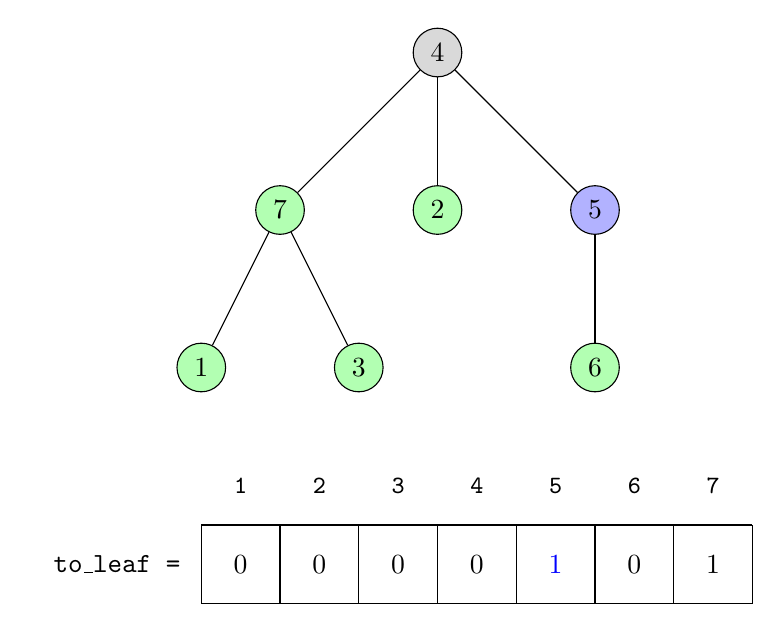
\begin{tikzpicture}

        \begin{scope}{shift={(3,0)}}
            \node[opacity=0] (X) at (-1, 0) { $1$ };

            \node[fill=gray!30,circle,draw] (D) at (4, 5) { $4$ };
            \node[circle,draw,fill=green!30] (C) at (2, 3) { $7$ };
            \node[circle,draw,fill=green!30] (E) at (4, 3) { $2$ };
            \node[circle,draw,fill=blue!30] (F) at (6, 3) { $5$ };
            \node[circle,draw,fill=green!30] (A) at (1, 1) { $1$ };
            \node[circle,draw,fill=green!30] (B) at (3, 1) { $3$ };
            \node[circle,draw,fill=green!30] (G) at (6, 1) { $6$ };

            \draw (A) -- (C);
            \draw (B) -- (C);
            \draw (C) -- (D);
            \draw (D) -- (E);
            \draw (D) -- (F);
            \draw (F) -- (G);

            \node[anchor=west] at (-1.0, -1.5) { \texttt{to\_leaf = } };
            \draw (1, -2) grid (8, -1);

            \node at (1.5, -0.5) { \small \texttt{1} };
            \node at (2.5, -0.5) { \small \texttt{2} };
            \node at (3.5, -0.5) { \small \texttt{3} };
            \node at (4.5, -0.5) { \small \texttt{4} };
            \node at (5.5, -0.5) { \small \texttt{5} };
            \node at (6.5, -0.5) { \small \texttt{6} };
            \node at (7.5, -0.5) { \small \texttt{7} };

            \node at (1.5, -1.5) { \textcolor{black}{$0$} };
            \node at (2.5, -1.5) { \textcolor{black}{$0$} };
            \node at (3.5, -1.5) { \textcolor{black}{$0$} };
            \node at (4.5, -1.5) { \textcolor{black}{$0$} };
            \node at (5.5, -1.5) { \textcolor{blue}{$1$} };
            \node at (6.5, -1.5) { \textcolor{black}{$0$} };
            \node at (7.5, -1.5) { \textcolor{black}{$1$} };

        \end{scope}
    \end{tikzpicture}

\end{frame}


\begin{frame}[fragile]{Visualização do algoritmo que computa \texttt{to\_leaf}}

    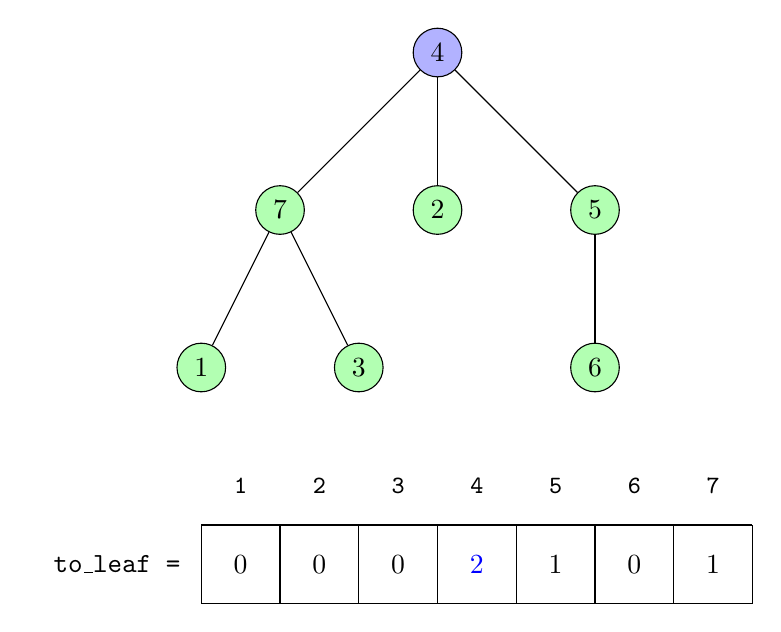
\begin{tikzpicture}

        \begin{scope}{shift={(3,0)}}
            \node[opacity=0] (X) at (-1, 0) { $1$ };

            \node[fill=blue!30,circle,draw] (D) at (4, 5) { $4$ };
            \node[circle,draw,fill=green!30] (C) at (2, 3) { $7$ };
            \node[circle,draw,fill=green!30] (E) at (4, 3) { $2$ };
            \node[circle,draw,fill=green!30] (F) at (6, 3) { $5$ };
            \node[circle,draw,fill=green!30] (A) at (1, 1) { $1$ };
            \node[circle,draw,fill=green!30] (B) at (3, 1) { $3$ };
            \node[circle,draw,fill=green!30] (G) at (6, 1) { $6$ };

            \draw (A) -- (C);
            \draw (B) -- (C);
            \draw (C) -- (D);
            \draw (D) -- (E);
            \draw (D) -- (F);
            \draw (F) -- (G);

            \node[anchor=west] at (-1.0, -1.5) { \texttt{to\_leaf = } };
            \draw (1, -2) grid (8, -1);

            \node at (1.5, -0.5) { \small \texttt{1} };
            \node at (2.5, -0.5) { \small \texttt{2} };
            \node at (3.5, -0.5) { \small \texttt{3} };
            \node at (4.5, -0.5) { \small \texttt{4} };
            \node at (5.5, -0.5) { \small \texttt{5} };
            \node at (6.5, -0.5) { \small \texttt{6} };
            \node at (7.5, -0.5) { \small \texttt{7} };

            \node at (1.5, -1.5) { \textcolor{black}{$0$} };
            \node at (2.5, -1.5) { \textcolor{black}{$0$} };
            \node at (3.5, -1.5) { \textcolor{black}{$0$} };
            \node at (4.5, -1.5) { \textcolor{blue}{$2$} };
            \node at (5.5, -1.5) { \textcolor{black}{$1$} };
            \node at (6.5, -1.5) { \textcolor{black}{$0$} };
            \node at (7.5, -1.5) { \textcolor{black}{$1$} };

        \end{scope}
    \end{tikzpicture}

\end{frame}

\begin{frame}[fragile]{Visualização do algoritmo que computa \texttt{to\_leaf}}

    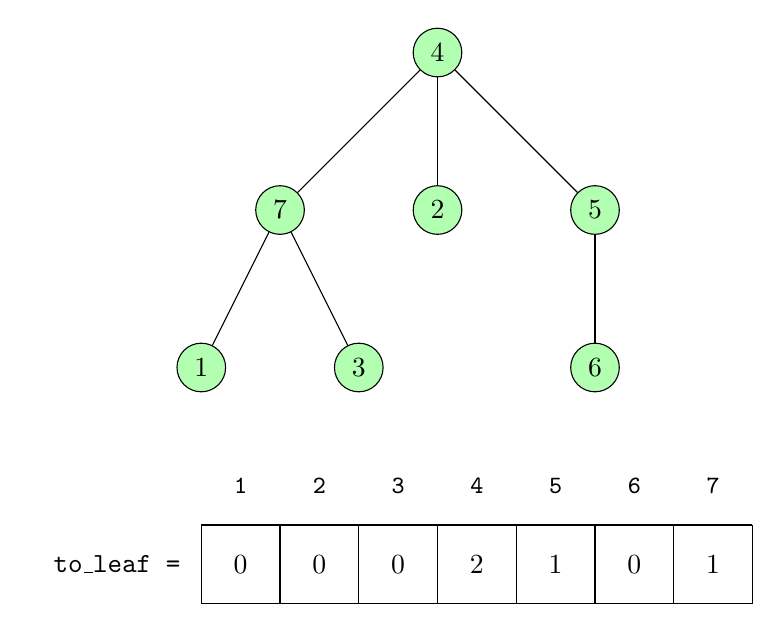
\begin{tikzpicture}

        \begin{scope}{shift={(3,0)}}
            \node[opacity=0] (X) at (-1, 0) { $1$ };

            \node[fill=green!30,circle,draw] (D) at (4, 5) { $4$ };
            \node[circle,draw,fill=green!30] (C) at (2, 3) { $7$ };
            \node[circle,draw,fill=green!30] (E) at (4, 3) { $2$ };
            \node[circle,draw,fill=green!30] (F) at (6, 3) { $5$ };
            \node[circle,draw,fill=green!30] (A) at (1, 1) { $1$ };
            \node[circle,draw,fill=green!30] (B) at (3, 1) { $3$ };
            \node[circle,draw,fill=green!30] (G) at (6, 1) { $6$ };

            \draw (A) -- (C);
            \draw (B) -- (C);
            \draw (C) -- (D);
            \draw (D) -- (E);
            \draw (D) -- (F);
            \draw (F) -- (G);

            \node[anchor=west] at (-1.0, -1.5) { \texttt{to\_leaf = } };
            \draw (1, -2) grid (8, -1);

            \node at (1.5, -0.5) { \small \texttt{1} };
            \node at (2.5, -0.5) { \small \texttt{2} };
            \node at (3.5, -0.5) { \small \texttt{3} };
            \node at (4.5, -0.5) { \small \texttt{4} };
            \node at (5.5, -0.5) { \small \texttt{5} };
            \node at (6.5, -0.5) { \small \texttt{6} };
            \node at (7.5, -0.5) { \small \texttt{7} };

            \node at (1.5, -1.5) { \textcolor{black}{$0$} };
            \node at (2.5, -1.5) { \textcolor{black}{$0$} };
            \node at (3.5, -1.5) { \textcolor{black}{$0$} };
            \node at (4.5, -1.5) { \textcolor{black}{$2$} };
            \node at (5.5, -1.5) { \textcolor{black}{$1$} };
            \node at (6.5, -1.5) { \textcolor{black}{$0$} };
            \node at (7.5, -1.5) { \textcolor{black}{$1$} };

        \end{scope}
    \end{tikzpicture}

\end{frame}

\begin{frame}[fragile]{Implementação da rotina que computa \code{c}{to_leaf[u]}}
    \inputsnippet{c++}{1}{21}{to_leaf.cpp}
\end{frame}

\begin{frame}[fragile]{Implementação da rotina que computa \code{c}{to_leaf[u]}}
    \inputsnippet{c++}{22}{42}{to_leaf.cpp}
\end{frame}


